% 
% Annual Cognitive Science Conference
% Sample LaTeX Paper -- Proceedings Format
% 

% Original : Ashwin Ram (ashwin@cc.gatech.edu)       04/01/1994
% Modified : Johanna Moore (jmoore@cs.pitt.edu)      03/17/1995
% Modified : David Noelle (noelle@ucsd.edu)          03/15/1996
% Modified : Pat Langley (langley@cs.stanford.edu)   01/26/1997
% Latex2e corrections by Ramin Charles Nakisa        01/28/1997 
% Modified : Tina Eliassi-Rad (eliassi@cs.wisc.edu)  01/31/1998
% Modified : Trisha Yannuzzi (trisha@ircs.upenn.edu) 12/28/1999 (in process)
% Modified : Mary Ellen Foster (M.E.Foster@ed.ac.uk) 12/11/2000
% Modified : Ken Forbus                              01/23/2004
% Modified : Eli M. Silk (esilk@pitt.edu)            05/24/2005
% Modified: Niels Taatgen (taatgen@cmu.edu) 10/24/2006

%% Change ``a4paper'' in the following line to ``letterpaper'' if you are
%% producing a letter-format document.

\documentclass[10pt,letterpaper]{article}

\usepackage{cogsci}
\usepackage{pslatex}
\usepackage{apacite}
\usepackage{graphicx}
\usepackage{float}
\usepackage{amsmath}

\title{The role of social information in cross-situational word learning}
 
\author{{\large \bf Kyle MacDonald (kyle.macdonald@stanford.edu)}} 


\begin{document}

\maketitle


\begin{abstract}
Social cues and the statistical regularity of language are both rich sources of information for word learners. Past research shows that social interaction facilitates language acquisition \cite{baldwin1995understanding, brooks2008infant} and in the absence of social information adults and children can track co-occurrence information to learn words \cite{blythe2010learning,smith2008infants}.  In the current study, I explore the interaction between these two information sources with a behavioral experiment and a computational model. The experiment added a social cue (eye gaze) to a cross-situational word learning task, changing the ambiguity of the initial learning episode. The model attempts to formalize how social information interacts with attention and generates predictions about human behavior in the experiment. I predicted that adding eye gaze would give learners more evidence about referential intent, allowing them to "explain away" spurious word-object mappings and reduce the need to track multiple referents for each word. Results suggest that learners were sensitive to the social cue, but did not change how they track multiple referents. Potential explanations for these results and future directions are discussed.  

\textbf{Keywords:} 
word learning; eye gaze; statistical learning; language acquisition
\end{abstract}


\section{Introduction}
To learn a new word\footnote{Here I will focus on the task of mapping words to objects with the goal of learning concrete nouns and assume that the learner has already solved the problem of word segmentation.}, the learner must solve several problems. She must simultaneously infer what is being talked about and the meaning of individual words in the speaker's utterance. This joint inference problem can be divided into two parts. The first involves making an inference about speaker's referential intent and the second making an inference about the links between words and objects. Together, these social-cognitive and mapping challenges make word learning a surprisingly difficult puzzle for the child to solve, and a great deal of research has tried to explain how children can learn words so rapidly.

To account for children's word learning skills, different theories of language acquisition emphasize different tools and information available to the learner. These proposals can be divided into two broad categories: \emph{Social-Pragmatic} and \emph{Associative} accounts. Social-Pragmatic theories characterize word learning as a result of children's social-cognitive skills and the highly structured learning moments created by adults (i.e. joint attentional frames).  Both experimental and observational data show that children possess sophisticated intention-reading skills, which they use in the service of word learning \cite{baldwin1993infants} and that episodes of joint attention facilitate word learning and vocabulary growth \cite{brooks2008infant}.  

In contrast, Associative accounts highlight the powerful statistical learning mechanisms that allow learner's to track the regularities of language, linking words and objects over time. In this account, word learning is best explained by domain-general pattern-finding abilities, attention, and memory. Several studies show that in the absence of social cues to word meaning, adults and children are able to rapidly learn words by tracking the co-occurrence of labels and objects across exposures \cite{smith2008infants,vouloumanos2008fine}. However, some researchers question the psychological plausibility of gradualist accounts, suggesting that children's rapid word learning is better described by a single hypothesis tracking mechanism \cite{trueswell2013propose,medina2011words}. 

Recent experimental work provides evidence that both adults and children can track and recall multiple referents and that this tracking interacts with attention and memory (Yurovsky & Frank, in prep). In Yurovsky and Frank's task, participants saw a set of novel objects and heard a novel word (e.g. Grink), and were asked to make a guess about the "correct"\footnote{There was actually no "correct" answers on exposure trials; rather these trials gave participants evidence about potential word-object mappings and allowed them to form an initial hypothesis.} word-object mapping. In subsequent test trials, participants heard the novel word again, this time paired with another set of novel objects. Critically, one of the objects in the set was either the participant's initial hypothesis (Same trials) or one of the objects that was \emph{not} the initial hypothesis (Switch trials). On Switch trials, adults reliably selected the object that was not their initial hypothesis, even when there were eight objects in the initial exposure set, providing strong evidence that learners track multiple referents when learning new words. 

However, this task did not include any of the rich social cues that typically accompany real world word learning. So it is still an open question as to how social information interacts with learners' demonstrated ability to track multiple referents. Perhaps the presence of additional evidence about a speaker's referential intent strengthens the learner's initial hypothesis, reducing the need to track alternative hypotheses. Or it could be that social information strengthens the initial hypothesis without reducing multiple referent tracking. The current study follows a recent line of research and modeling that attempts to integrate statistical and social learning\cite{johnson2012exploiting,frank2009using,yu2007unified}, and asks if the presence of social information changes how learners track multiple referents when learning new words?


%In this account, the puzzle of word learning is solved by children's sophisticated social-cognitive skills (e.g. intention-reading) and the highly structured situations in which children first learn words\cite{baldwin1995understanding,tomasello2009constructing}. These highly structured learning contexts (often called episodes of joint attention) are created by parents and involve shared attention to a handful of objects. These simplified learning contexts make the first inference about referential intent (i.e. the speaker's goals) easier, which in turn facilitates the mapping inference. Crucially, infants must possess the prerequisite intention-reading skills to sucessfully infer referential intent, even in these simplified contexts.

%A series of experimental work show the sophistication of children's early intention-reading skills (for a review, see \citeNP {tomasello2009constructing}). The common thread across these studies is that children could not have possibly relied on saliency and co-occurrence information to learn the novel word meanings. 

%Mike's intentional model. What does social information and assuming that language is communicative do for the learner? Discussion of the role of social information in learning: is it another weight in the computation or is it qualitatively different?

\section{Methods}

\subsection{Participants}

This experiment was posted to Amazon Mechanical Turk as a set of
Human Intelligence Tasks (HITs) to be completed only by participants with US IP
addresses that paid 30 cents each (for a detailed comparison of laboratory and Mechanical
Turk studies see \citeNP{crump2013evaluating}). 30 HITs were posted for each
condition (Social, Non-social) for total of 60 paid HITs. If a participant
completed the experiment more than once, he or she was paid each time but only data
from the first HITs completion was included in the final data set. In
addition, data was excluded from the final sample if participants did not give correct
answers for familiar trials (excluded 1 HIT).

\subsection{Stimuli}

Stimuli for the experiment consisted of black and white pictures of familiar
and novel objects, a schematic drawing of a human interlocutor, and audio recordings of familiar and novel words. Pictures of 32 familiar objects spanning a range of categories (e.g. squirrel, truck, tomato, sweater) were drawn from the set constructed by \citeA{snodgrass1980standardized}. Pictures of distinct but
difficult to name objects were drawn from the set of 140 first used in \citeA{kanwisher1997locus}. For ease of viewing on participants' monitors, pixel values for all pictures were inverted so that they appeared as white outlines on black backgrounds (see Figure 1). Familiar words consisted of the labels for the familiar objects as produced by AT&T Natural VoicesTM (voice: Crystal). Novel words were 1-3 syllable pseudowords obeying the rules of English phonotactics produced using the same speech synthesizer.

\begin{figure}[H]
	\centering
	\fbox{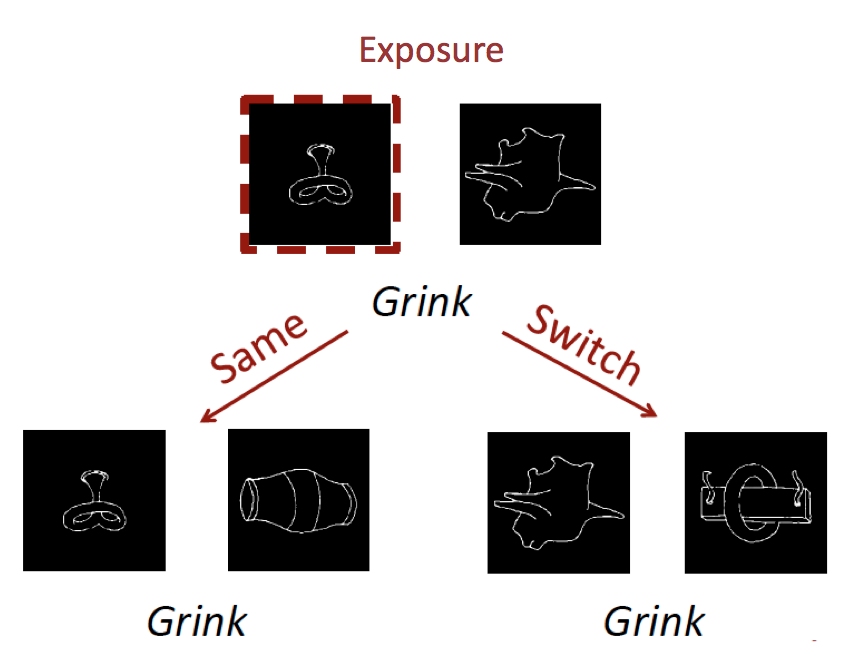
\includegraphics[scale=0.28]{stimuli2.png}}
	\caption{A schematic of the trials that participants saw in the experiment. On Exposure trials, participants saw four novel objects and heard a novel word. Participants were asked to guess it's correct referent. After the Exposure trial, participants either saw a Same or a Switch trial. On Same trials, the set of four referents contained the participant's previous hypothesis. On Switch trials, the set of referents contained one of the objects that the participants had \emph{not} hypothesized.}
\end{figure}

A schematic drawing of a human interlocutor was chosen for ease of manipulating the direction of eye gaze, the social cue of interest in this study. Five images were created using Adobe Photoshop with the following directions of eye gaze: far left, close left, close right, far right, and eyes center. The interlocutor's eyes were made larger and green arrows were added to cue subjects' attention to the direction of eye gaze\footnote{Because this task was performed over the internet and participants' screen sizes might be small, it was important to make the eye gaze cue clear.}.

\begin{figure}[H]
	\centering
	\fbox{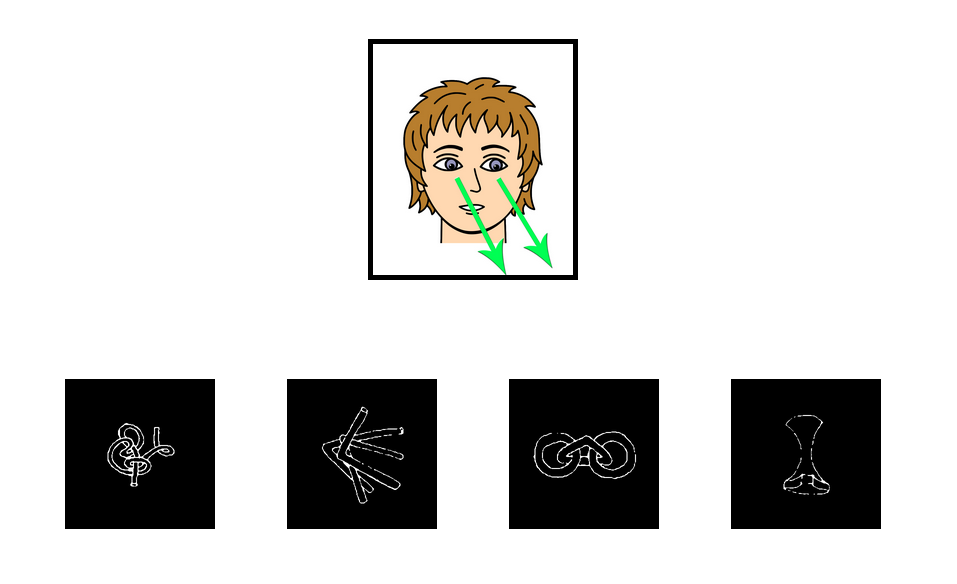
\includegraphics[scale=0.25]{stimuli1.png}}
	\caption{An example of an Exposure trial in the Social condition. In the Nonsocial condition, the interlocutor looked straight ahead during exposure. During test trials, the interlocutor looked straight ahead.}
\end{figure}

\subsection{Design and Procedure}

Participants were exposed to a series of trials in which they heard an interlocutor say a novel word, saw
four novel objects, and were asked to indicate their guess as to which object was the
referent of the word. After a written explanation of this procedure, participants were given
four practice trials to introduce them to the task. On each of these trials, they heard the interlocutor say a
Familiar word while looking at a line drawing of that object among a set of other familiar objects.
On the first two trials, participants were asked to find the squirrel, and the correct answer
was in the same position on each trial. On the next two trials, participants were asked to
find the tomato, and the correct answer switched positions from the first to the second
trial (in order to ensure that participants understood that the on-screen position was not
an informative cue to the correct target). These trials also served to screen for participants
who did not have their audio enabled or who were not attending to the task.

After these Familiarization trials, participants were informed that they would now hear
novel words, and see novel objects, and that they should continue selecting the correct
referent for each word. Participants each heard eight novel words twice. Participants saw four referents
on each trial, and the two trials for each word occurred back-to-back. Four of these
follow-up trials were Same trials in which the referent that participants selected on the exposure trial appeared again amongst the set of objects. The other four were
Switch trials in which one of the referents in the set was selected randomly from the objects
a participant did not select on the previous Exposure trial. All other referents were
completely novel on each trial. Critically, on Exposure trials the interlocutor's eye gaze was directed and thus informative, but on Same/Switch trials her eye gaze was undirected and thus uninformative. 

Participants were randomly assigned to one of two conditions: Social or Nonsocial. In the Social condition, eye gaze was informative on exposure trials. In the Nonsocial condition, eye gaze was uninformative throughout the task, i.e. the speaker always looked straight ahead. 

Because participants performed this task over the internet, it was important to
indicate to them that their click had been registered. Thus, a red dashed box appeared
around the object they selected for 1 second after their click was received. This box
appeared around the selected object whether or not it was the "correct" referent.

\section{Results and Discussion}

First, I compared the distribution of correct\footnote{A correct response for Same/Switch trials was selecting the referent that was present during Exposure trials.} responses to the distribution expected if participants were randomly selecting (defined by a Binomial distribution with four trials and a probability of success of $(\frac{1}{\#Referents}$). Figure 3 shows participants? accuracies in identifying the referent of each word in both conditions for both kinds of trials (Same and Switch). For both Same and Switch trials in both the Social and Nonsocial conditions, participants? responses differed from those expected by chance (smallest $\chi^{2}(4) = 12.07, p < .01$), replicating Yurovsky and Frank's finding that adults encode more than a single hypothesis in ambiguous word learning situations. 

\begin{figure}[H]
	\centering
	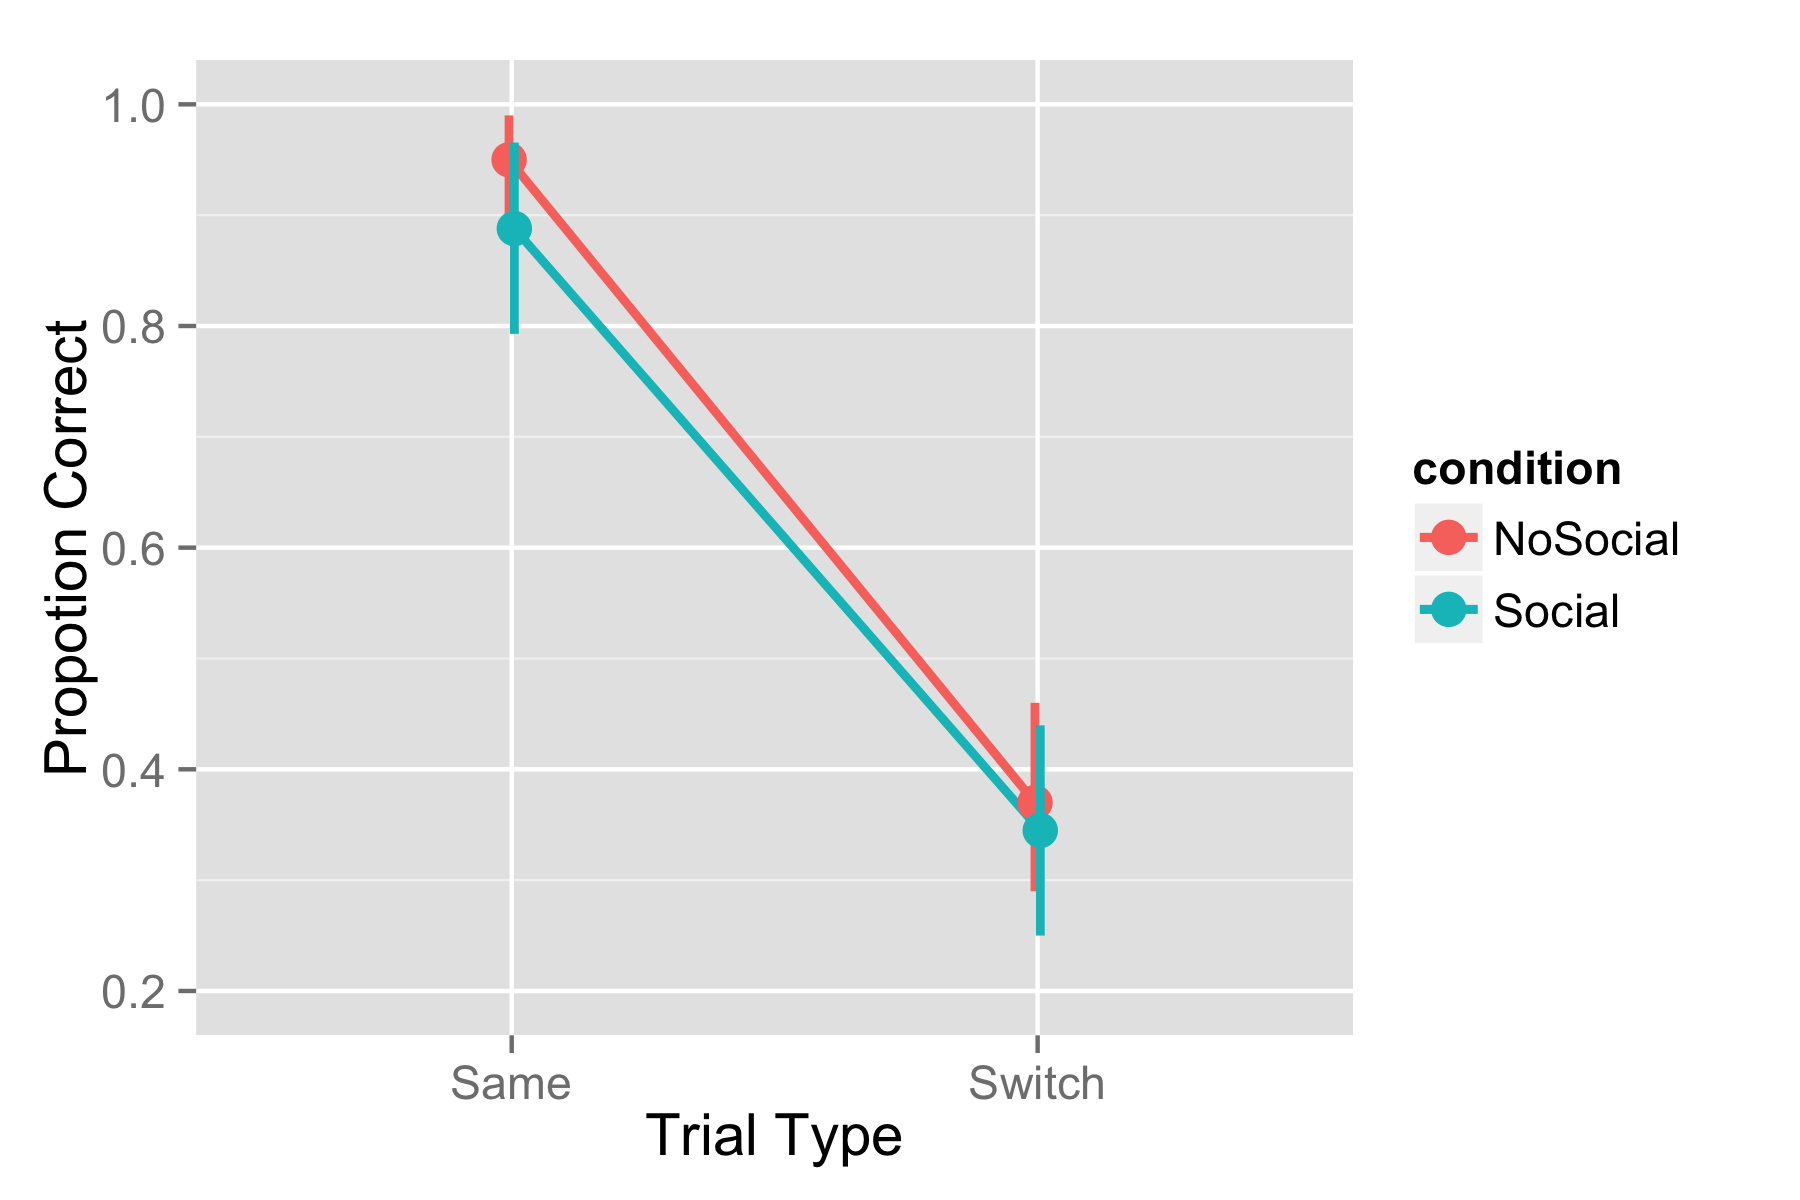
\includegraphics[scale=0.15]{accuracydark.png}
	\caption{Proportion of repeated referents selected by participants for each trial type (Same/Switch) and condition (Social/Nonsocial). Error bars indicate 95\% confidence intervals. Learning in all conditions differed from chance. There was no difference between the Social and Nonsocial conditions.}
\end{figure}

Next, I compared participants' performance on Same/Switch trials across conditions to see if the presence of a social cue during exposure changed participant's tracking of multiple referents. On both trail types, participants responses did not differ from each other: for Same trials, $ t(42) = -1.19, p > .05$, for Switch trials, $t(42) = -0.38, p > .05$. Thus, I did not find evidence that the presence of social information during exposure trials changed how participants tracked and recalled multiple referents on subsequent test trials.

To check if participants were actually sensitive to the speaker's eye gaze, I compared the distribution of correct responses \footnote{A correct response on Exposure trials is selecting the referent that was the target of the speaker's eye gaze.} on Exposure trials to the distribution expected if participants were selecting randomly. Participants' responses differed from those expected by chance, $t(239) = 16.89  p < .001$. Thus, there was evidence that participants were sensitive to the social cue and chose to use it, selecting the target of the interlocutor's eye gaze.

Finally, I explored participants' reaction times, comparing across conditions to see if the presence of social information altered the rate or participants' responses. Figure 4 shows participants' reaction time by trial and condition. Participants' responses did not differ on Same trials, $t(51) = 1.65, p > .05$. However, participants in the Social condition were slower on Switch trials, $t(51) = 2.63, p < .05$. This reaction time difference provides additional evidence that the presence of eye gaze had some effect on participants' behavior.

\begin{figure}[H]
	\centering
	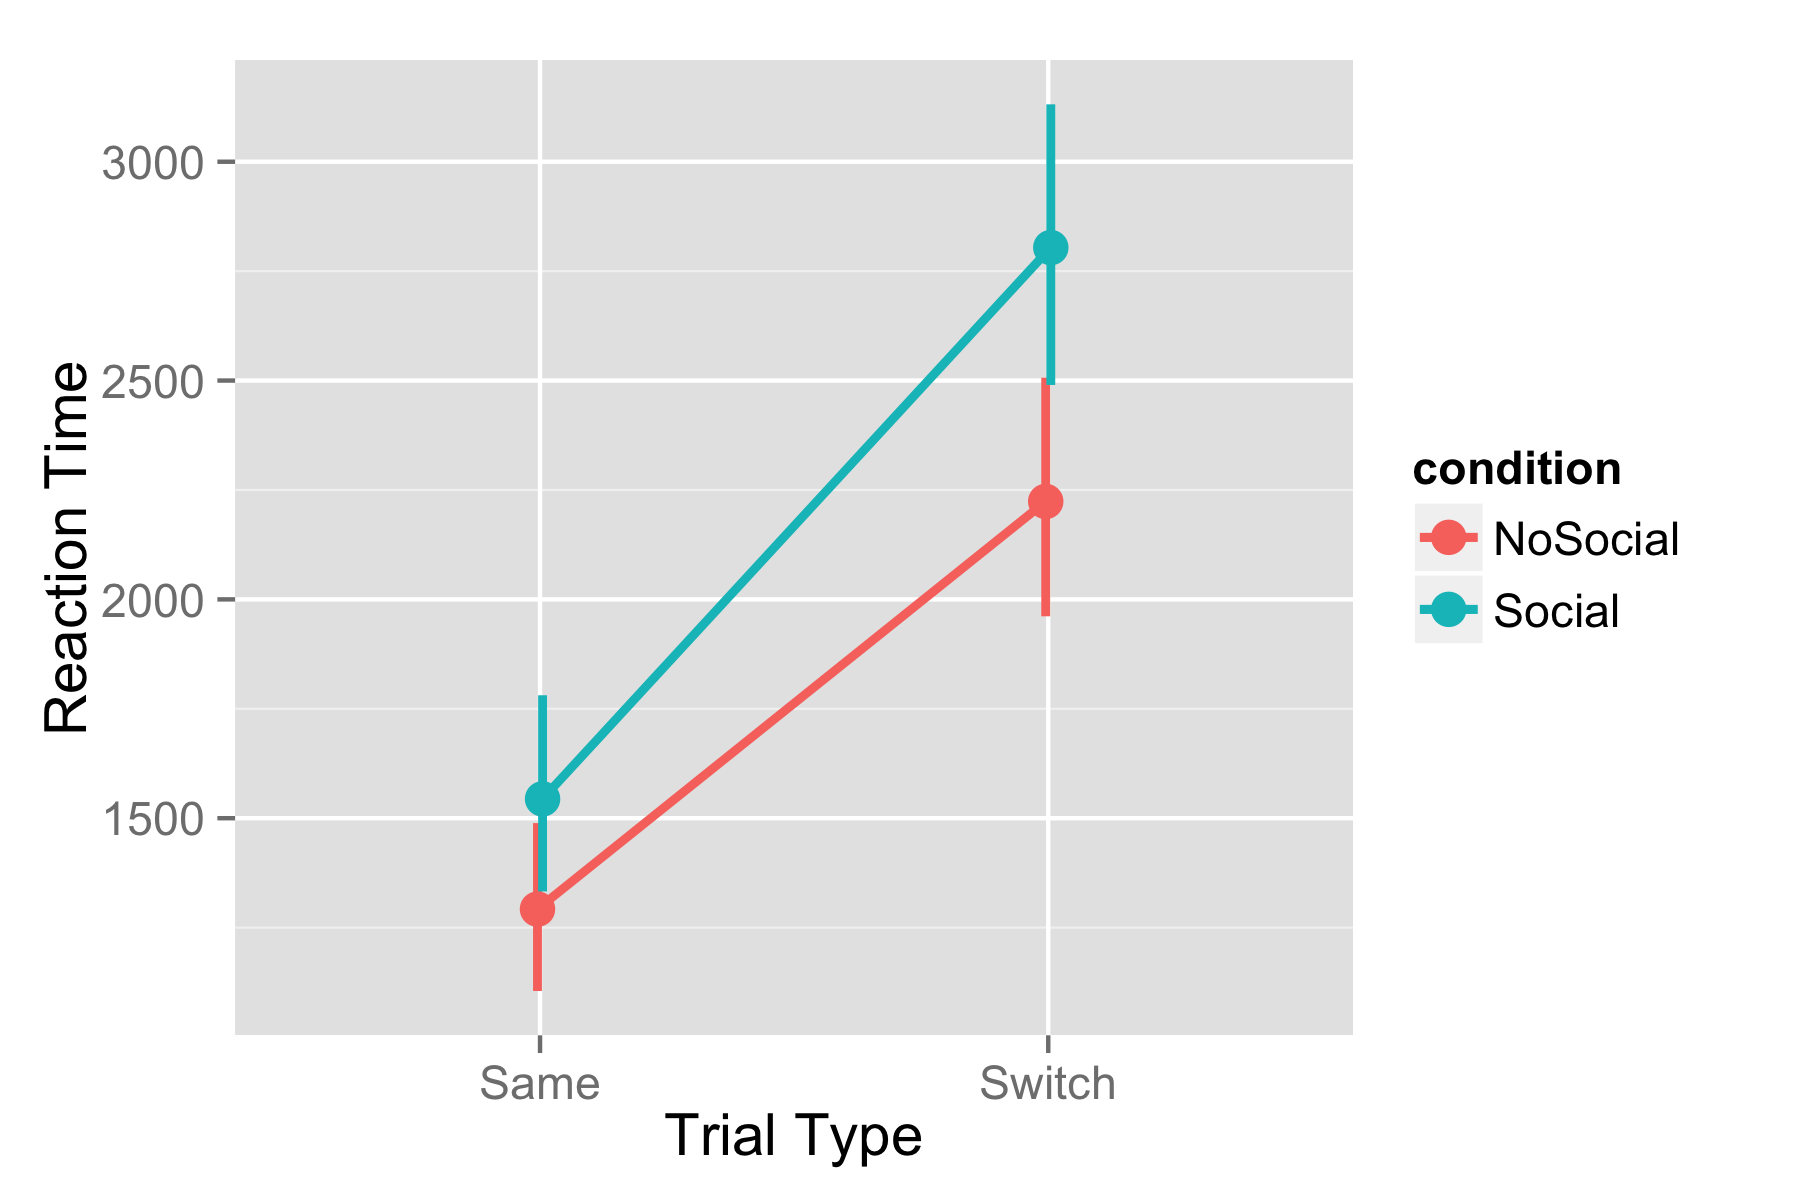
\includegraphics[scale=0.15]{rt.png}
	\caption{Reaction time for each trial type (Same/Switch) and condition (Social/Nonsocial). Error bars indicate 95\% confidence intervals. There was no difference between the Social and Nonsocial conditions on Same trials, but participants in the Social condition were slower to respond on Switch trials.}
\end{figure} 

Together, these results suggest that participants were sensitive to the interlocutor's eye gaze, selecting the target of her gaze on Exposure trials and responding more slowly on Switch trials in the Social condition. However, this sensitivity did not did not change how participants performed on accuracy in either Same/Switch trials. Potential explanations for these results and future directions are discussed below. 

\section{Conclusion and future work}

In this study, I investigated whether the presence of social information would change how adults track multiple word meanings. I predicted that eye gaze would provide additional evidence about the speaker's referential intent, strengthening the learner's initial hypothesis, potentially at a cost to tracking alternative hypotheses. The results did not provide evidence in support of this prediction. Adults tracked multiple hypotheses regardless of the presence of a social cue, but were slower to respond on Switch trials when social cues were present. 

The reaction time finding is somewhat interesting when you consider the structure of this cross-situational learning task. During Exposure trials, participants follow the speaker's gaze, often selecting the target as the "correct" referent. Then, participants are immediately confronted with a Switch trial in which the target of the interlocutor's gaze is no longer present. Perhaps participants slow reaction times are evidence of surprise that their initial hypothesis, which was weighted more strongly because of the presence of eye gaze, was no longer present. 

So why might participants show sensitivity to social information but still show evidence of tracking multiple hypotheses? The analysis of participants' initial hypotheses rules out the alternative explanation that participants did not pay attention to the social cue during exposure. However, it is possible that the combination of a static/schematic interlocutor and the lack of a natural sentence frame (e.g. "There's a X") caused the task to be pragmatically strange, which might have led participants to discount the interlocutor as a source of evidence about word-object mappings. 

Another possibility is that limiting the social information to eye gaze resulted in a weak social cue that didn't cause participants to change how they tracked the other referents. Recent research suggests that eye gaze might be a noisy and unreliable cue to reference \cite{frank2013social}. Future versions of the task could include stronger cues such as pointing or holding the object during Exposures trials to see if stronger evidence would alter learning. Future versions could also include more complex Exposure trials and more trials between exposure and test (similar to Yurovsky & Frank, in prep) to see how social information interacts with attention and memory demands. 

Language is a powerful tool that once mastered allows us to share our beliefs and learn from others. But learning a language is a surprisingly difficult challenge at several different levels. Thus, it is likely that language learners use several tools to take advantage of the sources of information available to them, both social and statistical. This study follows recent work that attempts to integrate social and statical learning with the hope that future studies will increase both our understanding of the unique contribution of each and how they interact to support learning. 

\bibliographystyle{apacite}

\setlength{\bibleftmargin}{.125in}
\setlength{\bibindent}{-\bibleftmargin}

\bibliography{fyp_p}


\end{document}
